% !TEX root = DesignDocument.tex

\chapter{System  and Unit Testing}

\section{Overview}
This section describes the approach we are taking with regards to system and unit testing. This section provides a brief overview of our testing approach, the testing frameworks we will use, and a description of how the testing will be done to ensure that our system will be successful.

Most of the testing for this project was done in Sprint 5

\section{Dependencies}
The testing dependencies for our project components are as followed:
\begin{itemize}
\item Web application - Microsoft Visual Studio Testing Framework
\item Web API - Microsoft Visual Studio Test Explorer
\item Tablet application - Espresso testing framework
\item Tablet application - JUnit
\end{itemize}


\section{Test Setup and Execution}

\subsection{Web Application Unit Testing}
The unit tests for the Web App project will be contained in a C\# project under the DoorPanes Visual Studio solution. The testing project will contain a testing class for every endpoint controller in the normal C\# project. Each testing class will contain methods that will test every endpoint method in the normal C\# project. The unit tests will be run in Microsoft Visual Studio. The dashboard controller contains the following endpoints that can be unit tested:

\begin{itemize}
\item Index Endpoint - Shows the main page of the dashboard controller. Will be unit tested under the conditions of being authorized, not authorized, and simple navigation to the controller.
\item Get Events Endpoint - Gets all endpoints from the database. 
\item Insert Event Endpoint - Saves events created on the Web App into the SQL database.
\item There are various other endpoints that the JavaScript code calls, but most of it just returns existing data.
\end{itemize}

\noindent ASP.NET MVC unit tests directly call methods of your MVC controllers. When a unit test calls an action method in a controller, you can validate that the correct view is returned (although you do not validate the HTML) and that view data is returned. You can also test whether a method correctly redirects to another controller or view.

\subsection{Web API Unit Testing}
Microsoft Visual Studio allows the user to create an accompanying test project when creating an API project.  The above section describing the general idea of how the web application was unit tested also applies to how the web API was unit tested. Also Moq was used to  mock repositories and databases for unit testing. The following endpoints in the web API that are unit tested:

\begin{itemize}
\item Login
\item Get Calendar Events
\item Get Calendar Events By Range and Owner
\item Get Calendar Events By Range and Room
\item Get Calendar Events By Owner
\item Get Calendar Events By Room
\item Get A Calendar Event
\item Get All Owners
\item Get All Rooms
\item Delete All Calendar Events
\end{itemize}

\subsection{Tablet Application Unit Testing}
All unit testing for the tablet application for this project will be done using the JUnit testing framework.  JUnit is a JAR file linked in at compile time under the package junit.framework. All unit tests will follow the format listed in the code shown.
\lstinputlisting[language=Java]{test.java}

Unit tests for the tablet application have been written to test the login function of the application.  These tests use the Espresso testing framework for Java/Android. This is an automated UI testing framework.  The tests are written in a test file and when run, user input is emulated and run on the application.  You can see the user inputs specified in the test be displayed during the run of the test.  Every thought of input for the login screen will be inputted to make sure the application handles the errors correctly.  Invalid usernames and passwords are checked to make sure that a correct message and prompt is displayed to the user.  On correct input, the test will check that the application moves to the correct activity.

As mentioned above, Espresso is a UI testing framework.  Because of this, all UI elements can be tested.  These include all buttons, menus, etc.  The testing framework can act as the user and "press" all the buttons and menus in the program.  The test will check to make sure the appropriate action is taken after each UI interaction	

\begin{figure}
  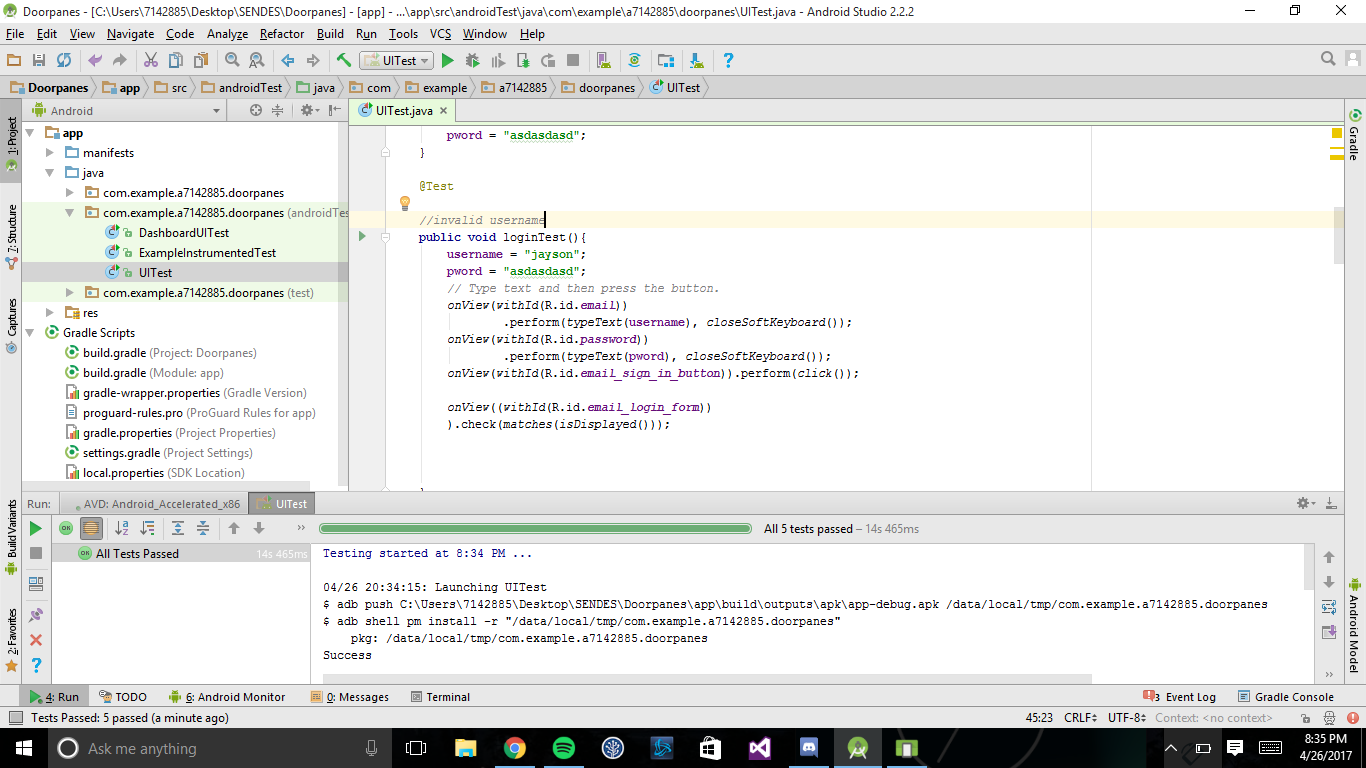
\includegraphics[width=\linewidth]{tablettest.png}
  \caption{Example of what a unit test looks like for the log in page.  You can see at the bottom of the page that all tests were successful!}
  \label{fig:tablettesting}
\end{figure} 

\section{System Testing}

One of the nice things about using Microsoft Azure is that performance testing, 	volume testing, stress testing, and scalability testing are all handled on the Microsoft Azure end. We don't have any control over the actual server hardware. All we would have to do is pay a higher price for more performance.\\

\noindent The following tests will be done to ensure the application is properly system tested.

\begin{itemize}
  \item GUI Testing - all parts of the interface will be tested to make sure the function and work properly.
  \item Usability testing - monitor how user uses the application and receive feedback based on there use of the program.
  \item Compatibility testing - make sure the application runs on all required versions of Android OS.
\end{itemize}

\section{System Integration Analysis}
For this project to work correctly, the tablet application needs to integrate the Web API calls.  API calls will be used to transfer data to and from the tablet application. To make sure all of these calls are working correctly and the system is properly integrated, tests will be written using JUnit, a Java testing framework.

\section{Risk Analysis}

\subsection{Web Application Risk Analysis}
There are no known risks that are under our control for the web application at this time.
\subsubsection{Risk Mitigation}
In terms of system risk analysis, we are  dependent on Microsoft for this. Hopefully Microsoft does a good job safeguarding the entrances to their data-centers and such.\\\\
\noindent
Possible risks for the web app include the risk of someone knowing a person's schedule. This could potentially increase the danger towards a person's safety. 

\subsection{Web API Risk Analysis}
The Web API for our project brings a few risks to consider, including the risk of SQL injections and other forms of accessing the database without permission.

\subsubsection{Risk Mitigation}
Taking these risks into account we will need to make the necessary steps to ensure that no unauthorized access is permitted.

\subsection{Tablet Application Risk Analysis}
The biggest issue in the tablet application will be security.  Our application needs to correctly identify and authenticate a user, and only they or users with access to that data can view and modify it.  The tablet application uses token based authentication.  A username and password is sent in a POST request.  If valid, a token will be returned which allows a user to access all the secure API calls.



\subsubsection{Risk Mitigation}
Care needs to be taken here. As of this moment, passwords and usernames may be sent in plain text.  HTTPS needs to be put into affect on this project to ensure no passwords can be watched over the network.

\section{Successes, Issues and Problems}

This section describes our successes and failure when it comes to the testing part of the project.

% Section Author: Andrew Fagrey
\subsection{Web Application}
When tested, the Web application had the following successes, issues, and problems:\\\\
\subsubsection{Successes}
\begin{itemize}
\item The endpoint to get the events was used the most, and therefore tested the most. We were able to achieve 100\% code coverage on testing for the get events endpoint.
\item The constructor of the dashboard controller was also unit tested, and it's now working well.
\item It's also important to note that almost all of the code not in the dashboard controller was written by Microsoft, and therefore we did not write unit tests for their code.
\end{itemize}
\subsubsection{Issues}
\begin{itemize}
\item Due to being unfamiliar with the way the Visual Studio testing framework mocks database calls during testing and not having enough time to figure it out, the insert event endpoint didn't get unit tested. We did, however, did do a good job of making sure valid data was passed to the endpoint, so there's not a huge concern that the insert function will fail.
\item The other small endpoints in the controller that just returned data were not unit tested due to the fact that they just return data.
\end{itemize}
\subsubsection{Problems}
\begin{itemize}
\item Aside form not being able to get the insert event function working and not being able to understand how the mock framework testing works, we didn't have any serious issues.
\end{itemize}

Final Testing Screenshot Result

\begin{figure}[tbh] 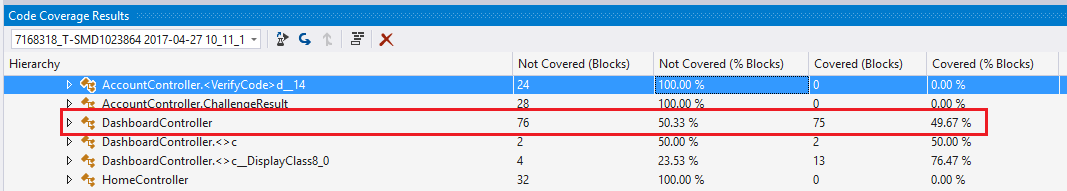
\includegraphics[scale=0.45]{./webAppCodeCoverage.png}
  \caption{Code Coverage for Dashboard Controller}
 \label{fig:webappCodeCoverage}
\end{figure}

\subsection{Web API}
When tested, the Web API had the following successes, issues, and problems:\\\\
Successes
\begin{itemize}
\item The controllers that were written for this project are 100\% unit tested and 98\% unit tested. The given code and controllers from Microsoft when creating the web API project was not unit tested
\end{itemize}
Issues
\begin{itemize}
\item Not all the controllers are 100\% unit tested.
\end{itemize}
Problems
\begin{itemize}
\item Figuring out how to throw certain exceptions while using Moq.
\end{itemize}
The following figures depict the unit test coverage results:

\begin{figure}[h!]
\centering
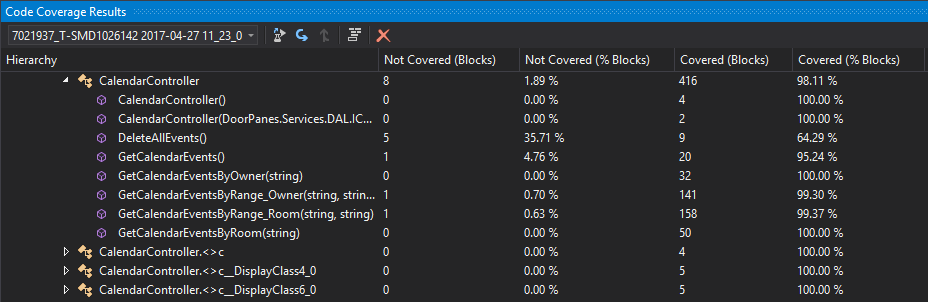
\includegraphics[width=0.75\textwidth]{./DetailCalendarCoverage.PNG}
\caption{Code Coverage for Calendar Controller}
\label{CalendarControllerCoverage}
\end{figure}

\begin{figure}[h!]
\centering
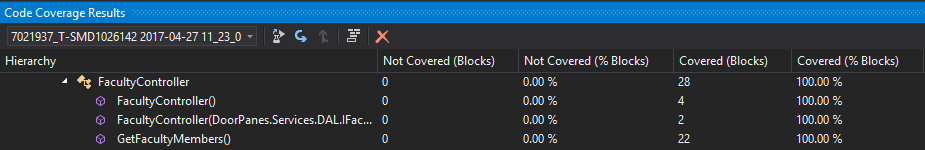
\includegraphics[width=0.75\textwidth]{./DetailFacultyCoverage.PNG}
\caption{Code Coverage for Faculty Controller}
\label{FacultyControllerCoverage}
\end{figure}

\begin{figure}[h!]
\centering
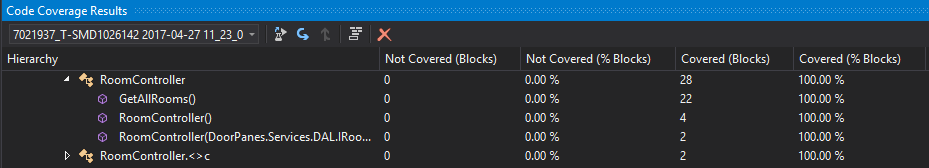
\includegraphics[width=0.75\textwidth]{./DetailRoomCoverage.PNG}
\caption{Code Coverage for Room Controller}
\label{RoomControllerCoverage}
\end{figure}

\subsection{Tablet Application}
When tested, the tablet application had the following successes, issues, and problems:\\\\
Successes
\begin{itemize}
\item Unit tested all possible inputs for log in page
\item Ran UI tests for all UI elements
\end{itemize}
Issues
\begin{itemize}
\item Unable to mock data that is being received using API calls.  So as of now it is assumed that the data coming in is correct and in the right format.
\end{itemize}
Problems
\begin{itemize}
\item Learning curve in making UI tests as it was unsure exactly how to test that.
\end{itemize}

